\documentclass[12pt,a4paper,oneside]{article}
\usepackage{afterpage,fullpage,amsmath,amsfonts,amssymb,amsthm}
\usepackage[cp1251]{inputenc}
\usepackage[english]{babel}
\usepackage{concrete}
\usepackage{euler}
\usepackage{ifthen}
\usepackage{cite}
\usepackage{soul}
\usepackage{listings}
%\usepackage[pdftex]{graphicx}
\usepackage{graphics}
\usepackage{graphicx}

\usepackage{algorithmic}
\usepackage{algorithm}
%\usepackage{cmap}
%\usepackage{tikz}

%\usepackage[T2A]{fontenc}
\usepackage[cp1251]{inputenc}
\newtheorem{problem}{Problem}
\newtheorem{theorem}{Theorem}
\newtheorem{definition}{Definition}
\newtheorem{remark}{Remark}
\newtheorem{lemma}{Lemma}
\title{Repeat resolving using paired data}
\author{Dmitry Antipov and Alexander Sirotkin}
%%-- \usepackage[14pt]{extsizes}

\def\eps{\varepsilon}

\begin{document}

\selectlanguage{english}
\maketitle

\begin{abstract}
 In this paper we give a general definition for validness of repeat resolving methods based on information, obtained from mate pairs. We introduce a class of operations on graphs that saves all possibilities to reconstruct genome and prove that the rectangle graph technique belongs to this class in case of error-free data. Furthermore, we provide some modifications of that technique which belongs to this class and provides better results than rectangle graph. In the last section we introduce an adaptation of our technique to non-errorless data. %, and how can inexact mate-read gaps be overcame.
\end{abstract}

\section{Motivation}
Most of sequencing machines provide not single reads, but mate-reads. We will show that mate-pair information can be used in more efficient way than modern assemblers do. It seems that right place for mate-pair information usage is repeat resolving step.
But to discuss different methods of repeat resolving based on paired information usage, we need to define what the correct repeat resolving method is and understand how we can compare quality different repeat resolving methods. 
In terms of graph the genome can be represented as a cycle (or path in case of non-cyclic genome). While applying different graph simplification methods we need to preserve this cycle.  

\section{About paired information}

Assume that we have a directed graph $G=(V,E)$ with specified lengths of all its edges. $G$ can be any abstract graph, but in case of genome assembling you may think that $G$ is compressed\footnote{Formal definition of compressing operation will be given later. Informally, for each vertex with only one incoming edge and only one outgoing edge we remove this vertex and concatenate this edges.} de Bruijn graph.  
For given edge $a$ we denote it's length as $l_a$. 
\begin{remark}
%In case of compressed de Bruijn graph with $k$-mers as vertices, length of edge is the number of nucleotides in this edge minus $k$. So the shortest possible edge is marked by $k+1$ nucleotides and it's length is one, by construction of compressed de Bruijn graph. 
In case of compressed de Bruijn graph with $k$-mers as vertices, length of edge is the number of $(k+1)$-mers in this edge.  
\end{remark}

\begin{definition}
Directed distance between two vertices $A$ and $B$ in directed path $P$, started in $A$ and finished in $B$, is the sum of the lengths of all edges in path $P$. 
%\begin{itemize}
%\item sum of edge length's, for edges situated between these instances %vertices
%in path, if $B$ is after $A$ in this directed path
%\item -distance($B$,$A$) in other case.
%\end{itemize}
\end{definition}

\begin{definition}
Directed distance between two edges $a$ and $b$ in directed path $P$ started from edge $a$ and finished by $b$ is sum of the lengths of all edges of $P$ with exception of $b$. 
%Given a directed path in graph, we define distance between two edges in this path as directed distance from start vertex of first edge to start vertex of second edge in this path.
\end{definition}

%In this approach we assume that vertices have not length.

For each edge $e$, we define $\mathop{start}(e)$ and $\mathop{end}(e)$ as start and end vertex of edge $e$ respectively. Length of path $P$ is sum of length of its edges (multiple occurrences allowed). We denote it as $|P|$.
For such graph we define \emph{edge pair} as ordered pair $(a, b)$ where $a \in E$ and $b \in E$.
\emph{Edge pair info} is a pair $((a, b), x)$ where $(a, b)$ is edge pair, and $x \in \mathbb{N}$.
\begin{definition}
For a given constant $d$ and path (or cycle) $P$ (from directed graph $G$), pair info $((a, b), x)$ is called \emph{$d$-consistent edge pair info with respect to $P$} if there exists directed subpath $P'$ of $P$, such that $P'$ starts from $a$, ends by $b$, $x$ is distance between $a$ and $b$ given by $P'$ and following inequalities hold\footnote{This condition guaranty us that in uncompressed graph there was a pair of edges with lengths one, with distance exactly $d$ between them, such that first edge was compressed into $a$ and second into $b$.
%������ ����� ������ � ����� $a$ ������� �����, � ������ � $b$.
}: $x - l_a \leq d$, $x + l_b \geq d$. 
\end{definition}

\begin{definition}
\emph{$d$-set of edge pair info} is set $S$ of edge pair infos such that there exists a Chinese postman cycle $C$ (possibly not unique)such that
 $((a, b), x) \in S \Leftrightarrow  ((a, b), x)$ is $d$-consistent with respect to cycle $C$.
\end{definition}
  
\subsection{Receiving paired info from reads}
It seems to be a subject of another paper...
\section{Repeat resolving}
We want to define what is ``correct'' graph transformation with respect to paired information and provide methods for comparison of these graph transformations in terms of the resulting graph complexity.

\subsection{Ungluings}
\begin{definition}
For given graph $G=(V, E)$, we say that graph $G' = (V', E')$  is an \emph{ungluing} of $G$ if there exists surjective mappings $f: V' \rightarrow V$ and $g: E' \rightarrow E$, $f$ and $g$ such that:
\begin{enumerate}
\item Edge length in $G'$ must be consistent with $g$ i.e. $\forall a\in E', l_a = l_{g(a)}$. 
% If $e'\in E'$ we define $\mathop{start_e}(e')$ as first edge from path $g(e')$
% and $\mathop{end_e}(e')$ as last edge from path $g(e')$.
\item $\forall e'\in E'\quad f(\mathop{start}(e')) = \mathop{start}(g(e'))$ i.e. $f\circ\mathop{start}=\mathop{start}\circ g$
\item $\forall e'\in E'\quad f(\mathop{end}(e')) = \mathop{end}(g(e'))$ i.e. $f\circ\mathop{end}=\mathop{end}\circ g$
\end{enumerate}
\end{definition}
\begin{remark}
For every \emph{ungluing} $G'$ of $G$ we can define gluing operation in terms of [Pevzner 2004] such that $G$ can be obtained as the result of performing this gluing operation to $G'$. This operation glues $f^{-1}(a)$ into $a$ for all $a\in V$, and $g^{-1}(e)$ into $e$ for all $e\in E$.
\end{remark}

\begin{definition}
\emph{Compress operation} for graph $G$ consists of following steps:
\begin{enumerate}
\item Select a vertex $A$ with in-degree and out-degree both equal to one. 
\item Remove the uniquely defined edges $a$ and $b$, with $\mathop{end}(a) = A$ and $\mathop{start}(b) = A$.
\item Remove vertex $A$.
\item Add edge $(\mathop{start}(a),\mathop{end}(b))$.% labeled by $ab$.
\end{enumerate} 
\end{definition}
\begin{definition}
For a given graph $G=(V, E)$, we say that a graph $G'' = (V'', E'')$ is a \emph{compressing} of $G$ if $G''$ is obtained from $G$ by any number of compress operation.
\end{definition}

\begin{remark}
For any edge from compressing $G''$ of $G$ we can find path in $G$ that is compressed into this edge. 
\end{remark}

\begin{definition}
For a given graph $G=(V, E)$, we say that a graph $G'' = (V'', E'')$ is a \emph{compressed ungluing} of $G$ if there exists an ungluing $G'$ of $G$, and $G''$ is compressing of $G'$.
\end{definition}

Till the end of this subsection, let $G=(V,E)$ be a graph, $G'=(V',E')$ - its ungluing and $G''=(V'', E'')$ -  compressed ungluing of $G$.  

\begin{definition}
For a given directed path $P' = (e'_0, \ldots, e`_n)$ in $G'$ we define \emph{decoding} of this path as $(g(e'_0), \ldots, g(e'_n))$ and denote it as $\mathop{dec}(P')$.
\end{definition}

\begin{definition}
For a given $d$-set $S$ of edge pair info and a cycle $C$ from graph $G$, $C$ is a \emph{valid} cycle iff $((a, b), x) \in S \leftrightarrow  ((a, b), x)$ is $d$-consistent with respect to cycle $C$.
\end{definition}
\begin{definition}  
We say that cycle $C'$ from graph $G'$ is \emph{valid} for a given $d$-set $S$ of edge pair info in graph $G$ if $dec(C')=C$ and $C$ is valid cycle in $G$.
\end{definition}
\begin{definition}  
For a given $d$-set $S$ of edge pair info in $G$, if $\mathop{dec}(\cdot)$ is a bijection between sets of valid cycles in $G$ and $G'$, we'll say that ungluing $G'$ is \emph{$S$-consistent ungluing}.
%We'll call such ungluing \emph{honest}.
\end{definition}

\begin{definition}  
For given $d$-set $S$ of edge pair info, if $G''$ is a compressing of any $S$-consistent ungluing of $G$, we'll say that $G''$ is \emph{$S$-consistent compressed ungluing}.
\end{definition}


\begin{remark}
  Note that ``ungluing'' is a graph notion that in general is independent on pair info. An ungluing $G'$ can be $S$-consistent with respect to one $d$-set $S$ of paired info and not $S$-consistent with respect to other one.
\end{remark}


\subsection{Informal reformulation}
Every valid cycle in $G$ corresponds to a variant of genome, consistent with graph and paired information. So, our condition means that any $S$-consistent ungluing is a transformation of $G$ which preserves all possibilities for genome from $G$ and does not produce any new possible genome cycles. 
\begin{remark}
The above definitions can be simply reformulated for linear genomes.
\end{remark}

%, every possibility for genome must be preserved, and no possible genomic cycle will transform to two different ones.


%\begin{remark}
%For given $\Delta$ we can slightly modify our condition about $d$-set of edge pair info.  We say that $\{(a_i, b_i), x_i\}$ is \emph{$(d, \Delta)$-set of edge pair info} if there exists $\{\delta_i\}$ where $\forall i \quad |\delta_i|\leq \Delta$ and $\{(a_i, b_i), x_i+\delta_i\}$ is $d$-set of edge pair info.
%\end{remark}
\subsection{Graph complexity estimation - still under discussion!}
\begin{problem}
  With given two $S$-consistent ungluings of a graph $G$, we want to define which one is somehow better.
\end{problem}
Let's consider an ungluing $G'= (V', E')$ of graph $G = (V, E)$. 
  For every vertex $v' \in V'$, we'll define \emph{vertex incoming-outgoing set} (and denote it as $O_{v'}$)  as $\{(a, b)| a\in E, b\in E\}$: $(a, b)$ satisfies following conditions:
\begin{enumerate}
 \item $\exists a' \in E' : \mathop{end}(a')=v', g(a') = a$
 \item $\exists b' \in E' : \mathop{start}(b')=v', g(b') = b$
\end{enumerate}
 We call vertex \emph{simple} if both in-degree and out-degree of this vertex both equal to one. Let's denote the set of simple vertices of graph $G'$ by $U_{G'}$. 
\emph{Graph incoming-outgoing set} is $\bigcup\limits_{v'\in E'\setminus U_{G'}}  O_{v'}$.
\emph{Measure of complexity} for $G'$ is the size of $G'$ graph incoming-outgoing set.
The complexity of any compressing of $G$ is equal to complexity of $G$.

There are many other possible measures, for example, minus sum of all edges length.

\section{Connection with rectangle graph}\footnote{We assume that basic concept of rectangle graph is known by reader.}

\begin{definition}
  \emph{Vertex pair info} is a triple $(A, B, x)$, where $A$ and $B$ are vertices and $x \in \mathbb{Z}$ 
\end{definition}
\begin{definition}
  \emph{Vertex-edge pair info} is a triple $(A, b, x)$, where $A$ is vertex, $b$ is edge and $x \in \mathbb{Z}$ 
\end{definition}
\begin{remark}
Labels of vertices in rectangle graph can be considered as vertex pair info.
\end{remark}

Let's consider using rectangle graph approach to simplifying our graph. 
There are three steps in it (without less of generality, we'll contract blue edges):
\begin{enumerate}
\item Building all possible rectangles.
\item Gluing vertices with same labels.
\item Contracting blue edges.
\end{enumerate}
Let's denote the resulting graph after all three steps as $G_r = (V_r,E_r)$ and result of first two steps as $G_{rb} = (V_{rb}, E_{rb})$. Each vertex $v_{rb}$ from $V_{rb}$ has a label - vertex pair info $(A(v_{rb}), B(v_{rb}), x(v_{rb}))$. We call first element of such triple \emph{first mark} of vertex $v_{rb}$ and denote it $\mathop{fm}(v_{rb})$. 

Since contracting of blue edges is a gluing operation, there exists a partition of $V_{rb}$ into family of disjoint subsets $\{H_{rb}(v_r)\}_{v_r\in V_r}$ such that all vertices from $H_{rb}(v_r)$ are glued into $v_r$. 
For a given vertex $v_r \in V_r$, let's consider $H_{rb}(v_r)$. Since two vertices from $G_{rb}$ connected by blue edge have same first mark, we can define mapping $f: V_r\rightarrow V$ by following equation:
$$f(v_r)=\mathop{fm}(v_{rb}), \text{ where }v_{rb}\text{ any element of } H_{rb}(v_r).$$

Each edge of $G_{r}$ has label from $E$ by construction. So this labeling provides us mapping $g:E_{r}\rightarrow E$. 

The conditions on $f$ and $g$ from definition of ungluing are satisfied by construction of rectangle graph.

\begin{remark}
  By construction, every vertex in one blue-connected component (set of vertices connected by blue edges) of $G_{rb}$ has the same vertex $V \in G$ as first mark.
\end{remark}

\begin{remark}
 The third step (contracting blue edges) is equivalent to constructing a graph with blue-connected components of $G_{rb}$ as vertex set. Two vertices in the new graph are connected with edge an labeled $e\in E$ iff in the corresponding connected components of $G_{rb}$ there are two vertices connected with an edge labeled $e$.  
\end{remark}

\begin{definition}
For given compressed de Bruijn graph $G=(V,E)$ and $d$-set of edge pair info $P$ 
we say that vertex pair info $(A, B, x)$ is \emph{obtained} from $P$ if there exists edge pair info $((a,b),y)$ such that:
\begin{itemize}
\item $a$ incoming edge for $A$, $b$ incoming edge for $B$ and $x=y-l_a+l_b$, 
\item $a$ outgoing edge for $A$, $b$ incoming edge for $B$ and $x=y+l_b$, 
\item $a$ incoming edge for $A$, $b$ outgoing edge for $B$ and $x=y-l_a$, 
\item $a$ outgoing edge for $A$, $b$ outgoing edge for $B$ and $x=y$. 
\end{itemize} 
\end{definition}
\begin{definition}
For given compressed de Bruijn graph $G=(V,E)$ and $d$-set of edge pair info $P$ 
we say that vertex-edge pair info $(A, b, x)$ is \emph{obtained} from $P$ if there exists edge pair info $((a,b),y)$ such that:
\begin{itemize}
\item $a$ is an incoming edge for $A$ and $x=y-l_a$, 
\item $a$ is an outgoing edge for $A$ and $x=y$. 
\end{itemize} 
\end{definition}
We denote such edge pair info $((a, b), y)$ (possibly not unique) as a \emph{precursor} of the vertex-edge pair info $(A, b, x)$.

\begin{definition}
Two vertex-edge pairs $(V,a,x)$ and $(V,b,y)$ are called \emph{adjacent} if $a$ and $b$ have at least one common\footnote{There are four possibilities: either $\mathop{start}(a)=\mathop{start}(b)$, either $\mathop{end}(a)=\mathop{start}(b)$, either $\mathop{end}(a)=\mathop{end}(b)$, either $\mathop{start}(a)=\mathop{end}(b)$.} vertex in graph $G$ and distances from $V$ to common vertices of $a$ and $b$, obtained from $(V,a,x)$ and from $(V,b,y)$, are the same. 
\end{definition}

We denote set of all vertex-edge pair infos obtained from $P$ as $P_v$. $P_v=\{(A,b,x)|A\in E, \exists (a,b,y)\in P: (a,b,y)\text{ is precursor for } (A,b,x)\}$
For vertex $Z\in E$, $P_v(Z) = \{(A, b, x)|(A, b, x) \in P_v; A = Z\}$.
 
Now we can define \emph{rectangle split operation}. This operation split one vertex at time. If we start from any graph $G$, and apply this operation consecutively we will obtain $G'$ that is $S$-consistent ungluing of $G$.

\begin{definition}
For a given vertex $Z \in V$ rectangle split operation consists of the following steps:
\begin{enumerate}
\item Partition $P_v(Z)$ into equivalence classes $C_i$ by the transitive closure of the adjacency relationship so that: $P_v(Z) = \bigcup C_i$. 
\item For each class $C_i$, create a vertex $Z_i$.
\item For each precursor $((a, b), y)$ of each vertex-edge pair info $(Z, b, x) \in C_i$,  create a copy $a_i$ of the edge $a$, replacing $start(a)$ (and resp. $end(a)$) with $Z_i$ iff $start(a)$ (resp. $end(a)$) $=Z$ and vertex-edge pair $(start(a), b, y)$ (resp. $(end(a)$) obtained from $((a, b), y)$ belongs to $C_i$.
\item For each precursor $((a, b), y)$ of each vertex-edge pair info $(Z, b, x) \in C_i$, replace $((a, b), y)$ in $P$ with $((a_i, b), y)$.
\item Remove $Z$ with all its incoming and outgoing edges.
\end{enumerate} 
\end{definition} 

\begin{remark}
   Step 3 is so complicated in definition because of loops. We need to replace $Z$ as start/end vertex of outgoing/incoming edge $a$, and also choose correctly only one of copies of $Z$ in case $a$ is a loop . 
\end{remark}

\begin{theorem}
  After applying rectangle split operation to each vertex of initial graph $G$ in any order we'll receive a graph $G' = (V', E')$, such that there exists one-to-one mapping from $(V', E')$ to $(V_r, E_r)$ and this mapping respects labeling.
\end{theorem}
\begin{remark}
 Initial graph $G$ is also correct ungluing of itself, with identical $f$ and $g$. We'll iteratively modify $f$ and $g$ in each rectangle split operation:
$f(Z_i):= f(Z)$, $g(a_i):= g(a)$
 It's evident, that after each rectangle split ungluing conditions (from definition of correct ungluing) on $f$ and $g$ are still satisfied.
\end{remark}
\begin{proof}
Let's fix some order of rectangle split operations.
While applying rectangle split operations to each vertex except $Z$, we can somehow modify $P$, but the set $P_v(Z)$ stays constant (because vertex-edge paired info, obtained from removed edge $e$ can be still obtained from an edge $e_i$ for some $i$). By construction of rectangle graph, there is a one-one mapping from $C_i$(and so from $Z_i$) to set of all blue-connected components, having $Z$ as first vertex in label. Let's consider union of this mappings for all vertices $Z \ in V$. 

Consider any edge $a_{ij}'=(Z_i, Y_j)$ with label $a$. 
Without losing of generality we can assume that vertex $Z$ of original graph $G$ split before $Y$. While splitting  $Y$, we have a precursor $((a_{i}, b), t)$ (that remapped into $(a_{ij}, b, t)$ ) of vertex-edge pair info's $(Y_j, b, t-l_{a_i}) \in D_j$, such that $\mathop{end}(a_{i}) = Y$ where $P_v(Y) = \bigcup D_j$. While splitting $Z$, we have a precursor $((a, b), t)$ of vertex-edge pair info's $(Z, b, t) \in C_i$, such that $\mathop{start}(a) = Z$. The edge pair info $((a, b), t)$ belongs to $C_i$ and $D_j$, this means that edge pair info $((a, b), t)$ produce rectangle such that red edges of this rectangle connect two blue edges  components that mapped into $C_i$ and $D_j$, and this edges labeled by $a$. So, we shown that for each edge in our graph $G'$ there exist an edge in $G_{rb}$ which respects one-one mapping on vertices and has the same label.

%If we take some edge from $G_{rb}$ then we can produce split operation like %above. But edge $b$ will be obtained from rectangle. And we produce sequence of %precursor $(a,b,t)\rightarrow (a_i,b,t))\rightarrow (a_{ij},b,t)$. This %sequence show as that in $G'$ exist edge connecting $Z_i$ and $Y_j$, and %labeled with $a$. 

Let's take red edge from $G_{rb}$ with label $a$. It connects two blue-connected components. These components are mapped to $C_i$ and $D_j$ from $G'$. Without less of generality, $Z$ was splitted before $Y$. So, by construction of $G'$, there exists an edge $b \in E$: such that $(Z, b, x)\in C_i$ and precursor of this vertex-edge pair is $((a,b),x)$. There is a vertex $Z_i \in G'$ mapped to $C_i$ in description of rectangle split operation. In step 4 of rectangle split operation, $((a, b), x)$ will be transformed into $((a_i,b),x)$. Then, consider the split of vertex $Y$. By construction, there exists $D_j$ :  $((Y,b),x-l_a) \in D_j$ for $((Y,b),x-l_a)$ obtained from $((a_i,b),x)$. After splitting $Y$, $a_i$ would be transformed into $a_{ij}$, where $\mathop{end}(a_{ij}) = Y_j$. So, we proved that after this two splits there'ld appear an edge $a_{ij}$ connecting $Z_i$ and $Y_j$, and no other splits wouldn't affect this edge.   
\end{proof}


\begin{theorem}
  In terms of Son's paper, result of his gluing procedure and contracting blue edges is a honest ungluing of initial graph $G$. 
\end{theorem}
\begin{proof}[sketch]
Each rectangle split operation for honest ungluing of $G$ produce honest ungluing of $G$, so if we apply them consequently, we'll receive a honest ungluing of $G$.
\end{proof}
\begin{theorem}
  In terms of Son's paper, result of his gluing procedure and contracting blue edges has measure of complexity, which is less or equal to measure of complexity of initial graph $G$. 
\end{theorem}
Each rectangle split operation  doesn't increase incoming-outgoing set(due to function $g$) of $G$, so their combination's incoming-outgoing set is also a subset of incoming-outgoing set of $G$.


\section{Our ideas}

\subsection{Bad cases for rectangle graph}
Rectangle graph is a powerful tool, but it's simple to construct graph that can be resolved manually, but stays unchanged after applying of rectangle graph techniques:
Lets consider graph $G$ with vertex set $V = {A,B,C,E,F,G,H}$ and edges $$\{(A,B),(B,C),(C,E),(E,F),(F,G),(G,A),(C,H),(H,F)\}$$. Pair information is set of all edge pairs with distance(on some subpath of $G$) 2 i.e. $(A,B)$ and $(C,E)$.
Both red and blue rectangle graph are isomorphic to $G$ but after using of slightly modified split operation for this graph we can receive a correct ungluing, consisting of two cycles: $(A\rightarrow B_1\rightarrow C_1\rightarrow E\rightarrow F_1\rightarrow G_1\rightarrow A)$ and $(A\rightarrow B_2\rightarrow C_2\rightarrow H\rightarrow F_2\rightarrow G_2\rightarrow A)$.

\subsection{Rectangle split modifications}
First approach is to modify adjacency definition for vertex-edge pairs.
\begin{definition}
 Two vertex-edge pairs $(Z,a,x)$ and $(Z,b,y)$ are called \emph{adjacent} if $ start (a) = end(b)\text{ or } start(b) = end (a)$ and distances from $Z$ to common vertices of $a$ and $b$, obtained from $(Z,a,x)$ and from $(Z,b,y)$, are same. 
\end{definition}
This definition  is slightly different from previous adjacency definition. Using this definition we can split vertex $V$ by vertex-edge information even if there two edges paired with $V$ has common start or end vertex.   

In case of inexact insert length we have to somehow weaken the condition on distances.
Also, for highly nonuniform coverage, the request of sharing vertex for adjacent edges should be weakened:

\begin{definition}
 Two vertex-edge pairs $(Z,a,x)$ and $(Z,b,y)$ are called \emph{$l-\eps$ adjacent} if there exists path $P$ from $a$ to $b$: $|P|<l$ and $||P| - |y-x|| < \eps$.   
\end{definition}

\subsection{Usage of split operations}

After performing rectangle split for all vertices of initial graph we can recalculate pair information and do split for new vertices. It can be useful if after splitting of all vertices from initial graph, some connected components of pair infos break into unconnected parts. 
Also, for some vertices it is possible to split them by using paired information in other direction - consider \emph{edge-vertex info} $(a, V, x)$ and look on adjacency(defined in same way as for vertex-edge infos) for such objects. This splitting is equivalent (in terms of rectangle graph) to contracting red edge. 

%\begin{tikzpicture}
%\Vertex[x=0,y=2.5]{A}
%\Vertex[x=0,y=5]{B}
%\Vertex[x=0,y=7.5]{C}
%\Vertex[x=-2.5,y=10]{E}
%\Vertex[x=0,y=12.5]{F}
%\Vertex[x=0,y=15]{G}
%\Vertex[x=2.5,y=10]{H}
%\Edge[style=->](A)(B)
%\Edge[style=->](B)(C)
%\Edge[style=->](C)(E)
%\Edge[style=->](E)(F)
%\Edge[style=->](F)(G)
%\Edge[style=->](G)(A)
%\Edge[style=->](C)(H)
%\Edge[style=->](H)(F)
%\end{tikzpicture}
%\subsection{Simple split operation}

%We start from graph $G_0$ and {$d$-set of edge pair info} $S$.
%We say that edge \emph{$e=(v_1, v_2)$ followed by $e'=(v_1', v_2')$ with respect to $S$} iff $v_2 = v_1'$ and 
%\begin{itemize}
%\item[either ] there exist edge $t$, and $x \in \mathbb{N}  $ such that $((e,t),x) \in S$ and $((e',t),x-l_e)\in S$; 
%\item[either ] there exist two edge $t=(w_1,w_2)$ and $t'=(w_2, w_3)$, and $x \in \mathbb{N}$ such that $((e,t),x) \in S$ and $((e',t'),x-l_e+l_t) \in S$. 
%\end{itemize}

%We say that edge \emph{$e$ close to $e'$ with respect to $S$} iff either $e$ followed by $e'$ with respect to $S$, either $e'$ followed by $e$ with respect to $S$.
%For each vertex $A$ we consider vertex incoming-outgoing set $S_A$ (defined above). We can divide $S_A$ in clusters $C_j$ due to transitive closure of \emph{close with respect to $S$} relationship, i.e. we build maximum as possible $C_j$ disjoint subsets of $S_A$ such that $S_A=\bigcup C_j$ and if two edge from $S_A$ are close with respect to $S$ than they belongs to one $C_j$.  

%Now we can define split operation for vertex $A$. We delete vertex $A$ and add new vertices $(A, C_j)$. For every incoming or outgoing $e$ edge we reroute it into vertex $(A, C_j)$ if $e\in C_j$. 


%Note, that we do not create ``new'' edges (there is evident bijection between edge sets in original and resulting graph), but split some vertices making graph simpler. 

%Such split operation not increase graph complexity measure defined above. 

\subsection{Incorporation of mate-read transformation (still under discussion!!!)}
Let's consider original rectangle split operation. 

After applying rectangle split operation to every vertex of initial graph we'll receive
graph $G'$ and a "hybrid" paired info- set of edge pairs, where first
element is an edge from $G'$, and second- an edge from $G$.

Let's translate it to terms of graph $G'$:
\begin{definition}
As \emph{paired multiedge info}
we'll call $((e_1, S_{e_2}), x)$, $e_1\in E',
S_{e_2}\subset E'$, saying that $\exists {e_2}_i \in S_{e_2}$ such that
distance between $e_1$ and $S_{e_2}$ is equal to $x$.
\end{definition}

If there is no path of length $x$ between $e_1$ and ${e_2}_i$, it means
that edge $e_1$ and ${e_2}_i$ are not in distance $x$, so in this case
${e_2}_i$ can be removed from $S_{e_2}$ !

We hope that such 'non-standart' mate-pair transformation
can be useful in repeat resolving.


So, now we forget about $G$ - every edge below  is edge from $G'$.
Also, we can remove all one-one vertices, merging it's incoming and outgoing edges and corresponging paired multiedge info

Then we can define vertex-multiedge pair info in similar way and
define adjacency for vertex-mutiedge pair info as something like
"There exists an edge $e_1$ from first edge-set and  $e_2$ from second
edge- set such that they share a vertex and distances to this vertex
provided from both pair infos are equal".

Now we can do an analogue of rectangle split operation with
vertex-multiedge pair info instead of vertex-edge pair info and
receive a graph $G''$

Again, it's easy to prove that it is honest ungluing.

Then again we can do the same with graph $G''$, and repeat this until
nothing is changed.
\begin{remark}
This method seems to be resistant to all  modifications of original rectangle split operation excluding ``back`` splitting.
\end{remark}
\section{Details about real implementation}
We have to ignore low confirmed information about distance between edges to cope with chimeric pairs. Also, it may turn out that after out resolving we'll need to do tip clipping again because of erroneous connections.

\section{Connected ideas}
\subsection{Insert-length distribution specifying}
We can use mate-pairs aligning the same edge to specify insert-length distribution.
\subsection{Complicated repeat resolving}
Next step is to resolve repeats using distances distributions on neighbouring edges (to divide sum of two close normal distributions with one). Also, in case of big coverage we can try to correct distance information. For example, we can obtain information about distances to vertex from distances to it's incoming and outgoing edges. This two series  of distances should be same. If they aren't, we can find minimal correction to get same distances and apply it to both of series.    
\subsection{Extending the model}
  In this paper we used only paired information. It seems that coverage can also be introduced to our model.
\section{Example}
Let's consider the graph on fig.~\ref{fig1}. Dotted lines connect edges on
distance ~d.
\begin{figure}
\begin{center}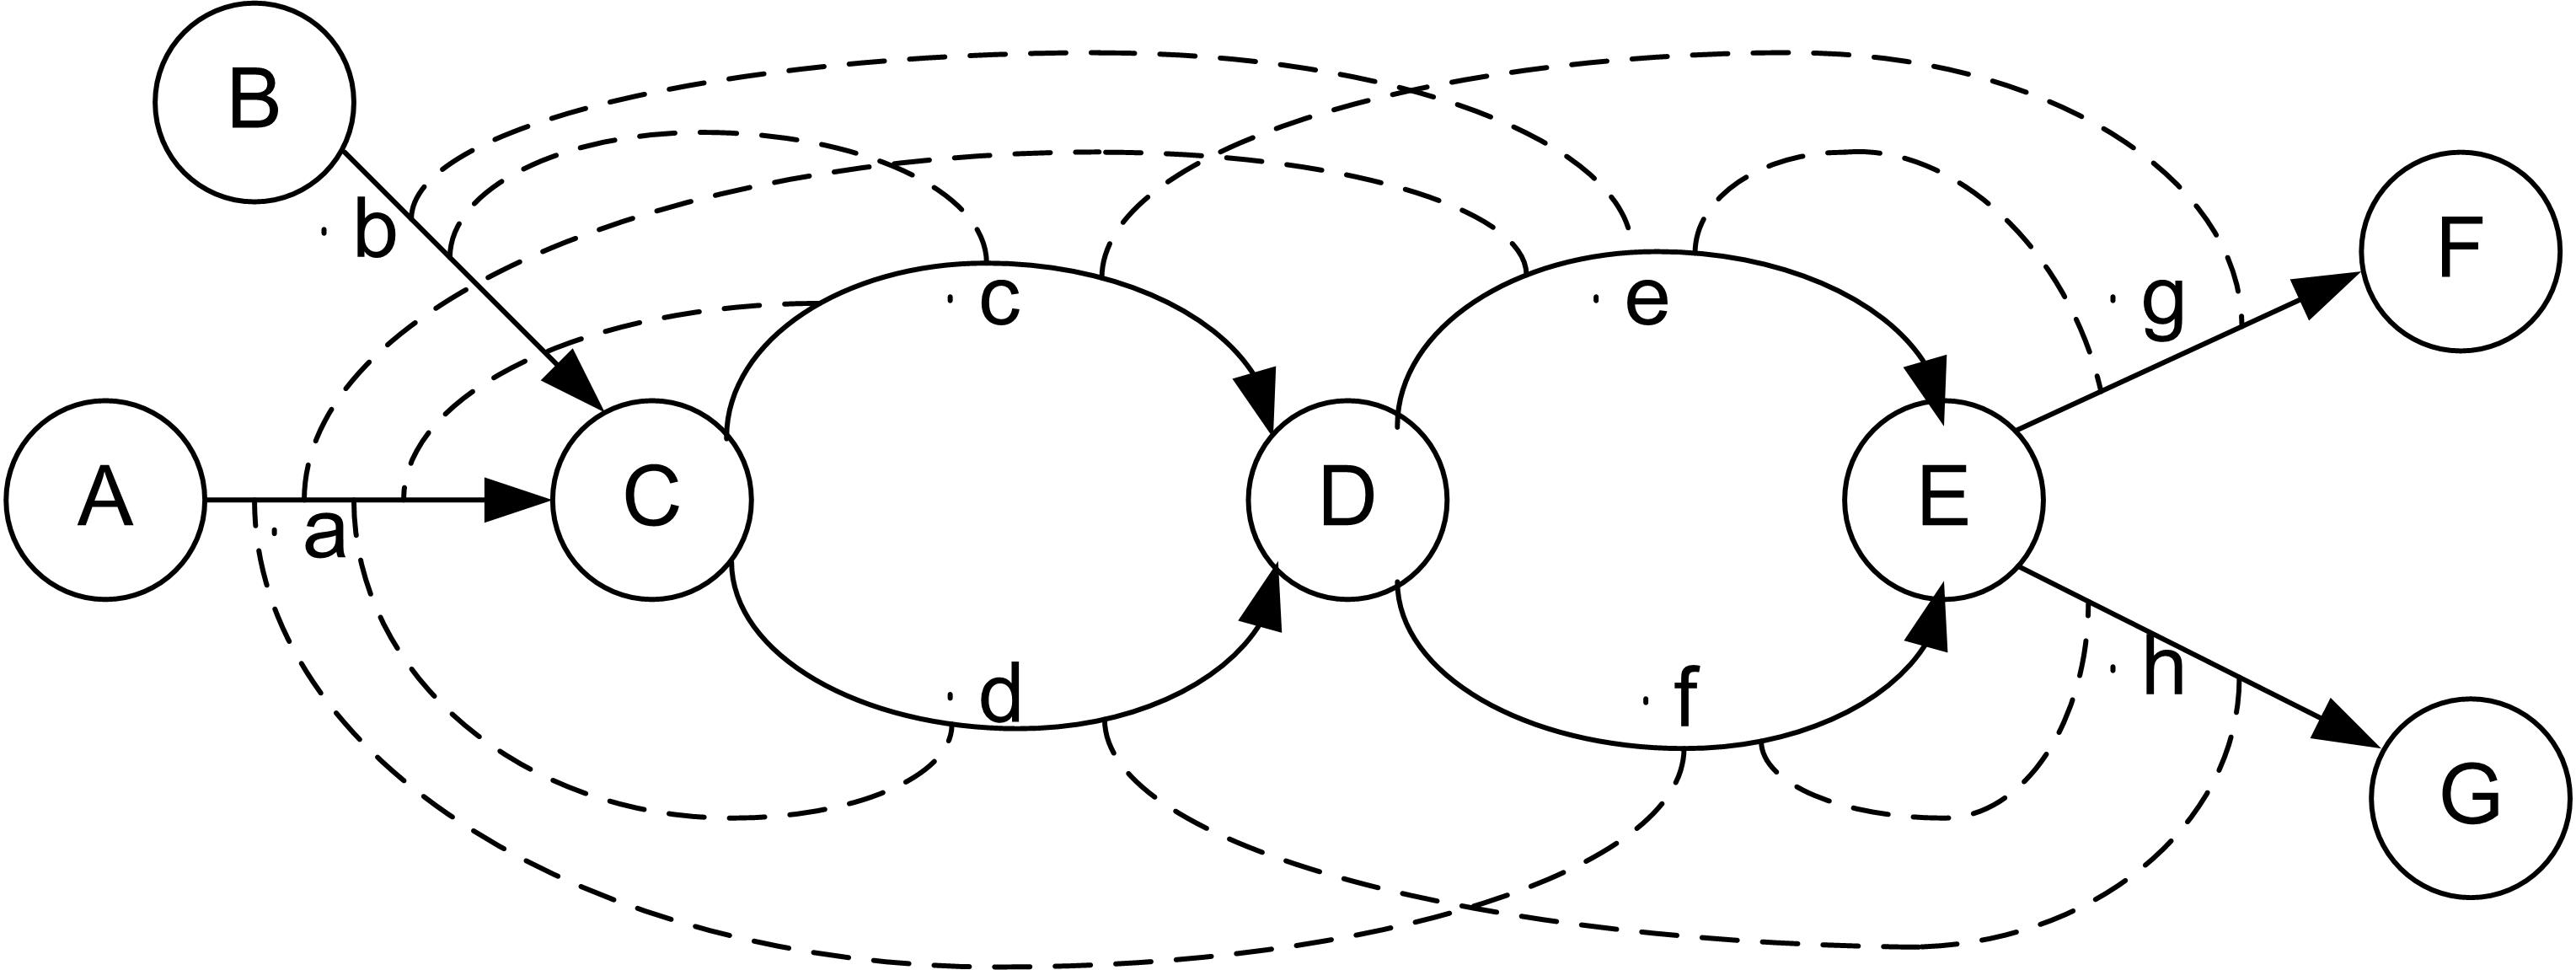
\includegraphics{jpg/Paired_Example.jpg}\end{center}
\caption{Graph example}
\label{fig1}
\end{figure}
Let's consider vertex $E$. The vertex-edge paired information obtained
from neighboring edges is $\{(E,g, 0),(E,h,0)\}$. In terms of rectangle
split operation this is one connected component, but in terms of our
slightly modified split operation there are two components. We split $E$
into $E_g$ and $E_h$, and edges remaps into this vertices as follow:
$e \rightarrow (D, E_g)$, $g \rightarrow (E_g,F)$, $f \rightarrow (D,E_h)$, $h \rightarrow (E_h, G)$.

Now let's consider vertex $C$. We obtain next set of vertex-edge pair
infos: $$\{(C,c,0), (C,e,l_c), (C,g,l_c+l_e), (C,d,0), (C,f,l_d),
(C,h,l_d+l_f)\}.$$ If lengths $l_c$ and $l_d$ are equal then all pair infos
above belong to one component. In this case we can not split anything.
Furthermore, there are no reasons to do this split if we know only
original graph and only this infos.

Let's see the vertex $D$. Infos are $\{(D,g,l_e),(D,h,l_f)\}$. By our rule
this set can be splitted into two components. For first component
$\{(D,g,l_e)\}$ we create vertex $D_g$, and have two precursors: $(c,g,*)$,
and $(e,g,*)$. So we remap edge $c$ into $(C, D_g)$, and $e$ into $(D_g, E_g)$.
For second component $\{(D,h,l_f)\}$ we have vertex $D_h$ and remap $d$ into
$(C,D_h)$ and $f$ into $(D_h,E_h)$.

Now we can return to vertex C. Set of vertex-edge pair infos is the
same $$\{(C,c,0), (C,e,l_c), (C,g,l_c+l_e), (C,d,0), (C,f,l_d),
(C,h,l_d+l_f)\}.$$
But now edge $c$ and edge $f$ no more adjacent, because $c$ remapped into
vertex $D_g$, but $f$ remapped into vertex $D_h$. The same happens with edges
$d$ and $e$. Now we have TWO component $\{(C,c,0), (C,e,l_c),
(C,g,l_c+l_e)\}$, and $\{(C,d,0), (C,f,l_d), (Cset of information,h,l_d+l_f)\}$. For first
component we create vertex $C_g$. We obtain next remapping of edges: $a
\rightarrow (A, C_g)$, $b \rightarrow (B, C_g)$, $c \rightarrow (C_g, D_g)$.
For second component we create vertex $C_h$ and obtain remapping $a \rightarrow
(A, C_f)$, $d \rightarrow (C_f, D_f)$. For both this component we remap edge $a$.
And now we have two edge marked by $a$.

So we split all possible vertices.

\end{document}

%Old stuff
 

%Imperfect 
%Fix some k.
%We define GEN, as ordered set of k-mer. This set can be represented as graph where vertices is position $i$ in GEN, labeled by k-mer on this position. Edges in this graph is $(i,i+1)$. Later if we say GENOME, we mean this graph. 

%We can define different gluing operation for GENOME. If we glue all vertices labeled with identical k-mers we got de Bruijn graph.

%If we have some glued graph we can want to obtain original graph. Lets try to do it by splitting glued vertices and edges. If we try to do this we found that with out new information it cant be done. As this new information we consider set of edge pair infos. For this type of infos we try to define some splitting rules.   

%  De bruijn group provides us compressed graph and paired data - set of somehow ordered distances between edge pairs, confirmed by reads. 
%We'll provide de-bruijn graph with some repeat resolving.
%For each edge(of compressed de bruijn graph) $x$ we 'll consider set $S_x: \forall y\in E,  y\in S_x \iff $ we have at least one mate-read such that left read in pair aligns to $x$ and right to $y$.
